\documentclass[preprint,12pt,authoryear]{elsarticle}

\usepackage{amsmath}
\usepackage{booktabs}
\usepackage{graphicx}
\usepackage[hidelinks]{hyperref}
\usepackage{lineno}
\linenumbers

% written by build_values_figures.py, do not edit
\newcommand{\vaggAgree}{98.6}
\newcommand{\vaggKappa}{0.91}
\newcommand{\valBlockNull}{0.757}
\newcommand{\valBlockRep}{0.850}
\newcommand{\valTempNull}{0.874}
\newcommand{\valTempNullSeventeen}{0.877}
\newcommand{\valTempRep}{0.864}
\newcommand{\vapBaseFive}{0.302}
\newcommand{\vapBaseFiveHi}{0.355}
\newcommand{\vapBaseFiveLo}{0.248}
\newcommand{\vapBaseTen}{0.255}
\newcommand{\vapBaseTenHi}{0.301}
\newcommand{\vapBaseTenLo}{0.209}
\newcommand{\vapBaseTwenty}{0.192}
\newcommand{\vapBaseTwentyHi}{0.236}
\newcommand{\vapBaseTwentyLo}{0.153}
\newcommand{\vapHgbFive}{0.411}
\newcommand{\vapHgbFiveHi}{0.469}
\newcommand{\vapHgbFiveLo}{0.351}
\newcommand{\vapHgbTen}{0.321}
\newcommand{\vapHgbTenHi}{0.376}
\newcommand{\vapHgbTenLo}{0.266}
\newcommand{\vapHgbTwenty}{0.213}
\newcommand{\vapHgbTwentyHi}{0.269}
\newcommand{\vapHgbTwentyLo}{0.167}
\newcommand{\vapNullFive}{0.767}
\newcommand{\vapNullFiveHi}{0.802}
\newcommand{\vapNullFiveLo}{0.729}
\newcommand{\vapNullTen}{0.658}
\newcommand{\vapNullTenHi}{0.704}
\newcommand{\vapNullTenLo}{0.610}
\newcommand{\vapNullTwenty}{0.500}
\newcommand{\vapNullTwentyHi}{0.559}
\newcommand{\vapNullTwentyLo}{0.446}
\newcommand{\vapRfFive}{0.408}
\newcommand{\vapRfFiveHi}{0.465}
\newcommand{\vapRfFiveLo}{0.347}
\newcommand{\vapRfTen}{0.320}
\newcommand{\vapRfTenHi}{0.375}
\newcommand{\vapRfTenLo}{0.264}
\newcommand{\vapRfTwenty}{0.227}
\newcommand{\vapRfTwentyHi}{0.284}
\newcommand{\vapRfTwentyLo}{0.178}
\newcommand{\vaquaAuc}{0.406}
\newcommand{\vaquaAucCtl}{0.440}
\newcommand{\vaquaAucCtlHi}{0.488}
\newcommand{\vaquaAucCtlLo}{0.397}
\newcommand{\vaquaAucHi}{0.468}
\newcommand{\vaquaAucLo}{0.345}
\newcommand{\vaquaCool}{24 of 31}
\newcommand{\vaquaCoolCtl}{24 of 31}
\newcommand{\vaucBaseFive}{0.779}
\newcommand{\vaucBaseFiveHi}{0.808}
\newcommand{\vaucBaseFiveLo}{0.751}
\newcommand{\vaucBaseTen}{0.743}
\newcommand{\vaucBaseTenHi}{0.773}
\newcommand{\vaucBaseTenLo}{0.711}
\newcommand{\vaucBaseTwenty}{0.657}
\newcommand{\vaucBaseTwentyHi}{0.703}
\newcommand{\vaucBaseTwentyLo}{0.612}
\newcommand{\vaucHgbFive}{0.843}
\newcommand{\vaucHgbFiveHi}{0.864}
\newcommand{\vaucHgbFiveLo}{0.823}
\newcommand{\vaucHgbTen}{0.791}
\newcommand{\vaucHgbTenHi}{0.814}
\newcommand{\vaucHgbTenLo}{0.767}
\newcommand{\vaucHgbTwenty}{0.642}
\newcommand{\vaucHgbTwentyHi}{0.692}
\newcommand{\vaucHgbTwentyLo}{0.593}
\newcommand{\vaucNullFive}{0.964}
\newcommand{\vaucNullFiveHi}{0.974}
\newcommand{\vaucNullFiveLo}{0.951}
\newcommand{\vaucNullTen}{0.934}
\newcommand{\vaucNullTenHi}{0.949}
\newcommand{\vaucNullTenLo}{0.918}
\newcommand{\vaucNullTwenty}{0.858}
\newcommand{\vaucNullTwentyHi}{0.888}
\newcommand{\vaucNullTwentyLo}{0.827}
\newcommand{\vaucRfFive}{0.842}
\newcommand{\vaucRfFiveHi}{0.862}
\newcommand{\vaucRfFiveLo}{0.821}
\newcommand{\vaucRfTen}{0.795}
\newcommand{\vaucRfTenHi}{0.818}
\newcommand{\vaucRfTenLo}{0.771}
\newcommand{\vaucRfTwenty}{0.686}
\newcommand{\vaucRfTwentyHi}{0.731}
\newcommand{\vaucRfTwentyLo}{0.640}
\newcommand{\vbandANull}{0.633}
\newcommand{\vbandANullHi}{0.649}
\newcommand{\vbandANullLo}{0.618}
\newcommand{\vbandAPrev}{0.888}
\newcommand{\vbandAPrevHi}{0.905}
\newcommand{\vbandAPrevLo}{0.871}
\newcommand{\vbandARf}{0.655}
\newcommand{\vbandARfHi}{0.682}
\newcommand{\vbandARfLo}{0.626}
\newcommand{\vbandARfWins}{20 of 31}
\newcommand{\vbandBNull}{0.687}
\newcommand{\vbandBNullHi}{0.703}
\newcommand{\vbandBNullLo}{0.673}
\newcommand{\vbandBPrev}{0.770}
\newcommand{\vbandBPrevHi}{0.801}
\newcommand{\vbandBPrevLo}{0.739}
\newcommand{\vbandBRf}{0.681}
\newcommand{\vbandBRfHi}{0.705}
\newcommand{\vbandBRfLo}{0.656}
\newcommand{\vbandBRfWins}{16 of 31}
\newcommand{\vbandCNull}{0.830}
\newcommand{\vbandCNullHi}{0.848}
\newcommand{\vbandCNullLo}{0.810}
\newcommand{\vbandCPrev}{0.653}
\newcommand{\vbandCPrevHi}{0.696}
\newcommand{\vbandCPrevLo}{0.607}
\newcommand{\vbandCRf}{0.716}
\newcommand{\vbandCRfHi}{0.740}
\newcommand{\vbandCRfLo}{0.692}
\newcommand{\vbandCRfWins}{1 of 31}
\newcommand{\vbandDNull}{0.968}
\newcommand{\vbandDNullHi}{0.981}
\newcommand{\vbandDNullLo}{0.954}
\newcommand{\vbandDPrev}{0.399}
\newcommand{\vbandDPrevHi}{0.450}
\newcommand{\vbandDPrevLo}{0.352}
\newcommand{\vbandDRf}{0.786}
\newcommand{\vbandDRfHi}{0.809}
\newcommand{\vbandDRfLo}{0.763}
\newcommand{\vbandDRfWins}{0 of 31}
\newcommand{\vbandENull}{0.991}
\newcommand{\vbandENullHi}{0.997}
\newcommand{\vbandENullLo}{0.984}
\newcommand{\vbandEPrev}{0.290}
\newcommand{\vbandEPrevHi}{0.335}
\newcommand{\vbandEPrevLo}{0.251}
\newcommand{\vbandERf}{0.850}
\newcommand{\vbandERfHi}{0.871}
\newcommand{\vbandERfLo}{0.829}
\newcommand{\vbandERfWins}{0 of 31}
\newcommand{\vbandFNull}{0.996}
\newcommand{\vbandFNullHi}{0.999}
\newcommand{\vbandFNullLo}{0.993}
\newcommand{\vbandFPrev}{0.219}
\newcommand{\vbandFPrevHi}{0.279}
\newcommand{\vbandFPrevLo}{0.174}
\newcommand{\vbandFRf}{0.889}
\newcommand{\vbandFRfHi}{0.908}
\newcommand{\vbandFRfLo}{0.869}
\newcommand{\vbandFRfWins}{0 of 31}
\newcommand{\vbcNull}{0.878}
\newcommand{\vbcNullMax}{0.888}
\newcommand{\vbcNullMin}{0.870}
\newcommand{\vbcRf}{0.917}
\newcommand{\vbufFolds}{155}
\newcommand{\vbufNullFive}{0.819}
\newcommand{\vbufNullFiveHi}{0.857}
\newcommand{\vbufNullFiveLo}{0.778}
\newcommand{\vbufNullOne}{0.943}
\newcommand{\vbufNullOneHi}{0.960}
\newcommand{\vbufNullOneLo}{0.924}
\newcommand{\vbufNullTen}{0.674}
\newcommand{\vbufNullTenHi}{0.777}
\newcommand{\vbufNullTenLo}{0.556}
\newcommand{\vbufNullTwo}{0.918}
\newcommand{\vbufNullTwoHi}{0.939}
\newcommand{\vbufNullTwoLo}{0.896}
\newcommand{\vbufRfFive}{0.647}
\newcommand{\vbufRfFiveHi}{0.688}
\newcommand{\vbufRfFiveLo}{0.606}
\newcommand{\vbufRfOne}{0.806}
\newcommand{\vbufRfOneHi}{0.832}
\newcommand{\vbufRfOneLo}{0.780}
\newcommand{\vbufRfTen}{0.576}
\newcommand{\vbufRfTenHi}{0.637}
\newcommand{\vbufRfTenLo}{0.526}
\newcommand{\vbufRfTwo}{0.765}
\newcommand{\vbufRfTwoHi}{0.794}
\newcommand{\vbufRfTwoLo}{0.735}
\newcommand{\vbufSkipFive}{23}
\newcommand{\vbufSkipOne}{0}
\newcommand{\vbufSkipTen}{144}
\newcommand{\vbufSkipTwo}{0}
\newcommand{\vbufWinsFive}{26 of 31}
\newcommand{\vbufWinsOne}{31 of 31}
\newcommand{\vbufWinsTen}{5 of 7}
\newcommand{\vbufWinsTwo}{31 of 31}
\newcommand{\vburnedMax}{4,896}
\newcommand{\vburnedMin}{515}
\newcommand{\vcaucBaseFive}{0.615}
\newcommand{\vcaucBaseFiveHi}{0.639}
\newcommand{\vcaucBaseFiveLo}{0.589}
\newcommand{\vcaucBaseTen}{0.609}
\newcommand{\vcaucBaseTenHi}{0.636}
\newcommand{\vcaucBaseTenLo}{0.582}
\newcommand{\vcaucBaseTwenty}{0.601}
\newcommand{\vcaucBaseTwentyHi}{0.632}
\newcommand{\vcaucBaseTwentyLo}{0.568}
\newcommand{\vcaucFive}{0.641}
\newcommand{\vcaucFiveHi}{0.663}
\newcommand{\vcaucFiveLo}{0.618}
\newcommand{\vcaucGain}{0.03}
\newcommand{\vcaucGap}{0.20}
\newcommand{\vcaucHgbFive}{0.638}
\newcommand{\vcaucHgbFiveHi}{0.659}
\newcommand{\vcaucHgbFiveLo}{0.617}
\newcommand{\vcaucHgbTen}{0.632}
\newcommand{\vcaucHgbTenHi}{0.654}
\newcommand{\vcaucHgbTenLo}{0.607}
\newcommand{\vcaucHgbTwenty}{0.608}
\newcommand{\vcaucHgbTwentyHi}{0.637}
\newcommand{\vcaucHgbTwentyLo}{0.578}
\newcommand{\vcaucTen}{0.632}
\newcommand{\vcaucTenHi}{0.659}
\newcommand{\vcaucTenLo}{0.605}
\newcommand{\vcaucTwenty}{0.610}
\newcommand{\vcaucTwentyHi}{0.643}
\newcommand{\vcaucTwentyLo}{0.576}
\newcommand{\vcellsMax}{41,730}
\newcommand{\vcellsMin}{2,544}
\newcommand{\vclosedDrop}{4}
\newcommand{\vclosedDropHi}{7}
\newcommand{\vclosedDropLo}{1}
\newcommand{\vclosedRelabel}{-11}
\newcommand{\vclosedRelabelHi}{-4}
\newcommand{\vclosedRelabelLo}{-22}
\newcommand{\vclosedStwo}{-28}
\newcommand{\vclosedStwoHi}{-13}
\newcommand{\vclosedStwoLo}{-46}
\newcommand{\vcurveFirst}{0.571}
\newcommand{\vcurveLast}{0.606}
\newcommand{\vcurveLastK}{30}
\newcommand{\vcurveTen}{0.601}
\newcommand{\venvQfive}{0.941}
\newcommand{\venvQfiveHi}{0.958}
\newcommand{\venvQfiveLo}{0.923}
\newcommand{\venvQone}{0.664}
\newcommand{\venvQoneHi}{0.694}
\newcommand{\venvQoneLo}{0.633}
\newcommand{\venvRise}{0.277}
\newcommand{\venvRiseHi}{0.307}
\newcommand{\venvRiseLo}{0.247}
\newcommand{\vexclCount}{4}
\newcommand{\vexclFires}{27}
\newcommand{\vexclNullWins}{27 of 27}
\newcommand{\vexclRise}{0.227}
\newcommand{\vexclRiseHi}{0.254}
\newcommand{\vexclRiseLo}{0.198}
\newcommand{\vfirecciFires}{8}
\newcommand{\vgateBand}{0.0000}
\newcommand{\vgateTransfer}{0.0005}
\newcommand{\vhistNull}{0.886}
\newcommand{\vhistNullHi}{0.910}
\newcommand{\vhistNullLo}{0.863}
\newcommand{\vhistRf}{0.814}
\newcommand{\vhistRfHi}{0.838}
\newcommand{\vhistRfLo}{0.791}
\newcommand{\vhistWins}{26 of 30}
\newcommand{\vitFolds}{51}
\newcommand{\vitNull}{0.515}
\newcommand{\vitRep}{0.813}
\newcommand{\vitRf}{0.801}
\newcommand{\vkoNull}{0.744}
\newcommand{\vkoRep}{0.829}
\newcommand{\vkoRf}{0.825}
\newcommand{\vlerrA}{5.4}
\newcommand{\vlerrAHi}{7.5}
\newcommand{\vlerrALo}{3.3}
\newcommand{\vlerrB}{2.5}
\newcommand{\vlerrBHi}{3.7}
\newcommand{\vlerrBLo}{1.4}
\newcommand{\vlerrC}{1.3}
\newcommand{\vlerrCHi}{1.8}
\newcommand{\vlerrCLo}{0.7}
\newcommand{\vlerrD}{0.7}
\newcommand{\vlerrDHi}{1.2}
\newcommand{\vlerrDLo}{0.4}
\newcommand{\vlerrE}{0.9}
\newcommand{\vlerrEHi}{1.6}
\newcommand{\vlerrELo}{0.3}
\newcommand{\vlerrF}{1.1}
\newcommand{\vlerrFHi}{2.3}
\newcommand{\vlerrFLo}{0.2}
\newcommand{\vlerrTenFarBand}{10.4}
\newcommand{\vlstAuc}{0.393}
\newcommand{\vlstAucCtl}{0.439}
\newcommand{\vlstAucCtlHi}{0.474}
\newcommand{\vlstAucCtlLo}{0.407}
\newcommand{\vlstAucHi}{0.434}
\newcommand{\vlstAucLo}{0.351}
\newcommand{\vlstCool}{26 of 31}
\newcommand{\vlstCoolCi}{16}
\newcommand{\vlstCoolCtl}{24 of 31}
\newcommand{\vlstCorr}{0.76}
\newcommand{\vlstCorrHi}{0.80}
\newcommand{\vlstCorrLo}{0.69}
\newcommand{\vlstHotCi}{2}
\newcommand{\vmeNull}{0.821}
\newcommand{\vmeNullPr}{0.697}
\newcommand{\vmePrev}{0.331}
\newcommand{\vmyBurned}{23.2}
\newcommand{\vmyBurnedHi}{28.2}
\newcommand{\vmyBurnedLo}{19.1}
\newcommand{\vmyCauc}{0.690}
\newcommand{\vmyCaucHi}{0.710}
\newcommand{\vmyCaucLo}{0.671}
\newcommand{\vmyNull}{0.887}
\newcommand{\vmyNullHi}{0.909}
\newcommand{\vmyNullLo}{0.864}
\newcommand{\vmyNullTen}{0.812}
\newcommand{\vmyNullTenHi}{0.845}
\newcommand{\vmyNullTenLo}{0.780}
\newcommand{\vmyRf}{0.812}
\newcommand{\vmyRfHi}{0.829}
\newcommand{\vmyRfLo}{0.795}
\newcommand{\vmyRfTen}{0.772}
\newcommand{\vmyRfTenHi}{0.794}
\newcommand{\vmyRfTenLo}{0.751}
\newcommand{\vmyRise}{0.241}
\newcommand{\vmyRiseFires}{31 of 31}
\newcommand{\vmyRiseHi}{0.268}
\newcommand{\vmyRiseLo}{0.214}
\newcommand{\vmyWins}{26 of 31}
\newcommand{\vmyWinsTen}{20 of 31}
\newcommand{\vnFires}{31}
\newcommand{\vnearDrop}{0.663}
\newcommand{\vnearDropHi}{0.692}
\newcommand{\vnearDropLo}{0.634}
\newcommand{\vnearMcd}{0.655}
\newcommand{\vnearRelabel}{0.636}
\newcommand{\vnearRelabelHi}{0.666}
\newcommand{\vnearRelabelLo}{0.603}
\newcommand{\vnearStwo}{0.612}
\newcommand{\vnearStwoHi}{0.643}
\newcommand{\vnearStwoLo}{0.579}
\newcommand{\vnullWinsFive}{31 of 31}
\newcommand{\vnullWinsHgbFive}{31 of 31}
\newcommand{\vnullWinsHgbTen}{31 of 31}
\newcommand{\vnullWinsHgbTwenty}{30 of 30}
\newcommand{\vnullWinsTen}{31 of 31}
\newcommand{\vnullWinsTwenty}{29 of 30}
\newcommand{\vpwdNullFive}{0.526}
\newcommand{\vpwdNullFiveHi}{0.531}
\newcommand{\vpwdNullFiveLo}{0.522}
\newcommand{\vpwdNullTen}{0.514}
\newcommand{\vpwdNullTenHi}{0.517}
\newcommand{\vpwdNullTenLo}{0.511}
\newcommand{\vpwdNullTwenty}{0.508}
\newcommand{\vpwdNullTwentyHi}{0.511}
\newcommand{\vpwdNullTwentyLo}{0.506}
\newcommand{\vrhoDist}{-0.07}
\newcommand{\vrhoDistHi}{0.05}
\newcommand{\vrhoDistLo}{-0.23}
\newcommand{\vrhoDom}{-0.07}
\newcommand{\vrhoDomHi}{0.06}
\newcommand{\vrhoDomLo}{-0.22}
\newcommand{\vrhoShift}{-0.12}
\newcommand{\vrhoShiftHi}{0.04}
\newcommand{\vrhoShiftLo}{-0.26}
\newcommand{\vrhoYear}{0.08}
\newcommand{\vrhoYearHi}{0.21}
\newcommand{\vrhoYearLo}{-0.04}
\newcommand{\vrise}{0.234}
\newcommand{\vriseFires}{31 of 31}
\newcommand{\vriseFiresHgb}{31 of 31}
\newcommand{\vriseHi}{0.261}
\newcommand{\vriseLo}{0.208}
\newcommand{\vtrAboveSix}{29.1}
\newcommand{\vtrBase}{0.545}
\newcommand{\vtrBaseHi}{0.552}
\newcommand{\vtrBaseLo}{0.538}
\newcommand{\vtrBelowHalf}{40.6}
\newcommand{\vtrDirections}{930}
\newcommand{\vtrFar}{0.532}
\newcommand{\vtrFarHi}{0.541}
\newcommand{\vtrFarLo}{0.522}
\newcommand{\vtrMinmax}{0.541}
\newcommand{\vtrMinmaxHi}{0.548}
\newcommand{\vtrMinmaxLo}{0.534}
\newcommand{\vtrNear}{0.526}
\newcommand{\vtrNearHi}{0.531}
\newcommand{\vtrNearLo}{0.521}
\newcommand{\vtrPoolMinmax}{0.601}
\newcommand{\vtrPoolMinmaxHi}{0.628}
\newcommand{\vtrPoolMinmaxLo}{0.574}
\newcommand{\vtrPoolRaw}{0.575}
\newcommand{\vtrPoolRawHi}{0.605}
\newcommand{\vtrPoolRawLo}{0.543}
\newcommand{\vtrPoolZ}{0.606}
\newcommand{\vtrPoolZFar}{0.634}
\newcommand{\vtrPoolZFarHi}{0.673}
\newcommand{\vtrPoolZFarLo}{0.595}
\newcommand{\vtrPoolZHi}{0.635}
\newcommand{\vtrPoolZLo}{0.578}
\newcommand{\vtrPoolZNear}{0.565}
\newcommand{\vtrPoolZNearHi}{0.593}
\newcommand{\vtrPoolZNearLo}{0.536}
\newcommand{\vtrRaw}{0.530}
\newcommand{\vtrRawHi}{0.537}
\newcommand{\vtrRawLo}{0.522}
\newcommand{\vtrSingle}{0.530}
\newcommand{\vtrSingleHi}{0.542}
\newcommand{\vtrSingleLo}{0.517}
\newcommand{\vtrZ}{0.553}
\newcommand{\vtrZHi}{0.560}
\newcommand{\vtrZLo}{0.546}


\journal{Environmental Modelling \& Software}

\begin{document}

\begin{frontmatter}

\title{A predictor-free geographic reference for evaluating wildfire susceptibility models, tested on 31 Mediterranean fires and five published datasets}

\author[cu]{Emrehan Metin}
\author[cu]{Yunus Emre Cogurcu\corref{cor1}}
\ead{ycogurcu@cu.edu.tr}
\cortext[cor1]{Corresponding author.}
\affiliation[cu]{organization={Department of Computer Engineering, Faculty of Engineering, \c{C}ukurova University},
            city={Sar\i\c{c}am, Adana},
            postcode={01330},
            country={T\"urkiye}}

\begin{abstract}
Wildfire susceptibility models are usually judged by the area under the receiver operating characteristic curve (AUC). Burned cells cluster in space, so part of that score may reflect where the fire is. We propose a protocol that compares every evaluation with a predictor-free model ranking cells by distance to training fires, reports a geography-calibrated AUC and rescores a fixed model on distance bands. On 31 Mediterranean fires the predictor-free model beat a random forest in \vnullWinsFive{} fires (AUC \vaucNullFive{} against \vaucRfFive{}). Calibration lowered the forest to \vcaucFive{}, and its AUC rose from \vbandARf{} to \vbandFRf{} as unburned cells lay farther from the fire. Sentinel-2 relabelling and a multi-year label did not remove these effects. In five published datasets the reference matched the reported model under a temporal split and fell to \vitNull{} under large blocks. Reporting it shows how much of a score the validation design explains.
\end{abstract}

\begin{graphicalabstract}
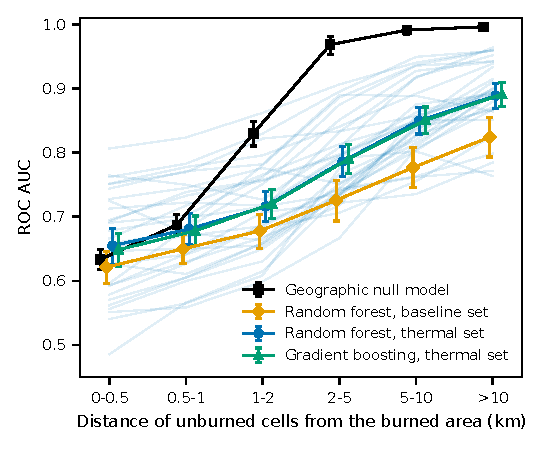
\includegraphics[width=\linewidth]{figures/Figure_2.pdf}
\end{graphicalabstract}

\begin{highlights}
\item A model with no predictors beat a random forest in 31 of 31 wildfires
\item Geography-calibrated AUC was 0.64 where the usual AUC was 0.84
\item AUC rose from 0.66 to 0.89 as test negatives moved away from the fire
\item Sentinel-2 relabelling did not explain the low AUC near the fire edge
\item The reference matched or beat a published model under a temporal split
\end{highlights}

\begin{keyword}
wildfire susceptibility \sep spatial cross-validation \sep null model \sep model evaluation \sep random forest \sep remote sensing
\end{keyword}

\end{frontmatter}

\section{Introduction}
\label{sec:intro}

Machine-learning maps of where wildfires are likely to burn are now common, and most of them are trained on burned areas or ignition points mapped from satellites and judged by the AUC on held-out cells. A review of 298 studies found that naive cross-validation on spatially dependent data is a recurring weakness of this literature \citep{Jain2020}. The best AUC reported in recent susceptibility papers is often above 0.9 \citep{Iban2022,Trucchia2023,Zerouali2026}.

Such numbers are hard to interpret because burned cells form contiguous patches. A test cell next to a burned training cell is easy to classify, and an unburned cell far from the fire is easy to reject, whatever the predictors say. Ecologists showed long ago that the choice of absence area changes AUC \citep{Lobo2008,VanDerWal2009}. \citet{Hijmans2012} went further and scored species distribution models against a null model that knows only the geographic distance to training presences. That null model beat MaxEnt for 45\% of 226 species. \citet{Ploton2020} found that a random forest given only coordinates matched an environmental model of forest biomass, and \citet{Meyer2018} and \citet{Roberts2017} showed how random cross-validation overstates performance on spatial data. In wildfire work, \citet{Zerouali2026} reported that AUC rose from 0.76 to 0.87 as pseudo-absences were drawn at least 0.5 to 2~km from fire points, and \citet{PhelpsWoolford2021} and \citet{Quan2023} discussed how fire occurrence models should be evaluated and how unburned labels should be sampled.

What is missing is a reference against which a wildfire susceptibility score can be read. None of the studies we found compares a fire model with a predictor-free geographic model, and the distance effect has been shown by retraining on different absence sets, which mixes a change in the model with a change in the test. It is also unknown whether the effect is an artefact of the coarse burned-area labels near the fire edge, which miss mixed pixels and unburned islands \citep{Boschetti2019}, and whether it carries over to the multi-year inventories that most susceptibility studies use.

This paper proposes and tests an evaluation protocol with three parts, a geographic null model in the sense of \citet{Hijmans2012}, a geography-calibrated AUC, and a rescoring of fixed out-of-fold predictions on disjoint distance bands. We apply it to 31 large Mediterranean fires mapped by MODIS MCD64A1, with a random forest and a gradient boosting model on vegetation, terrain and land surface temperature predictors. We check the edge labels against Sentinel-2, repeat the analysis with a multi-year label and rerun the null model on five published open datasets under their authors' own validation designs. Section~\ref{sec:methods} describes the data and the protocol, Section~\ref{sec:results} the results, Section~\ref{sec:discussion} what they mean for the evaluation of susceptibility models and Section~\ref{sec:conclusions} concludes.

\section{Data and methods}
\label{sec:methods}

The protocol needs a set of fires with a burned label and predictors on a common grid, a model to evaluate and a fixed validation design. Section~\ref{sec:fires} describes the fires and the data, Section~\ref{sec:models} the models and the validation, and Sections~\ref{sec:null} and \ref{sec:bands} the two parts of the protocol. Sections~\ref{sec:labels} to \ref{sec:secondary} describe the checks, and Section~\ref{sec:prereg} how the analysis was fixed in advance.

\subsection{Fires and data}
\label{sec:fires}

The fires are the five Mediterranean regions of an earlier study (Manavgat 2021, Bej\'is 2022, Mu\u{g}la 2021, North Evia 2021 and Montiferru 2021) and 26 further fires from 2017 to 2023 selected by rule from MCD64A1 \citep{MCD64A1}. The rule took the largest burned-area clusters of the Mediterranean summer season, kept those whose burned cells were mostly natural vegetation and dropped clusters overlapping one already chosen. For each fire, a 58-day predictor window ends the day before the first burn date of the dominant event, and a 49-day label window starts on that day. The study rectangle is the extent of the labelled cells plus 0.15\textdegree{}.

All inputs were processed in Google Earth Engine \citep{Gorelick2017} by one open pipeline \citep{ThermalTwinRepo} and aggregated to cells of about 500~m. A cell is burned if MCD64A1 records a burn date inside the label window, and cells that burned before the window are excluded. The predictors are the Normalised Difference Vegetation Index (NDVI), elevation and slope from the Copernicus DEM \citep{CopernicusDEM}, land cover from ESA WorldCover \citep{Zanaga2022} and six thermal predictors derived from Landsat 8 \citep{LandsatC2L2} and MODIS MOD11A1 \citep{MOD11A1}. The thermal predictors are the land surface temperature (LST) of the predictor window, its anomaly against earlier years, a temperature-vegetation dryness index and its change, and a downscaled and a gap-filled LST. The population of each fire is the set of valid cells dominated by tree, shrub or grass cover. The 31 fires hold between \vcellsMin{} and \vcellsMax{} such cells and \vburnedMin{} to \vburnedMax{} burned ones.

\subsection{Models and validation}
\label{sec:models}

The model under evaluation is a random forest \citep{Breiman2001} with 300 trees, a minimum leaf size of 3 and balanced class weights, trained either on a baseline set (NDVI, elevation, slope, land cover) or on the baseline set plus the six thermal predictors. A histogram gradient boosting classifier with 300 iterations on the thermal set is the second model. Missing values are filled with the training median. Each fire is evaluated separately with five-fold cross-validation stratified by label and grouped by square blocks of 10, 20 and 40 cells (about 5, 10 and 20~km). The 5~km blocks are the main design. We report ROC AUC and the average precision (PR-AUC), and means over fires carry a 95\% interval from 2,000 bootstrap resamples of fires.

\subsection{Geographic null model and calibrated AUC}
\label{sec:null}

The geographic null model uses no predictor. In each fold it scores a test cell by minus its distance to the nearest burned cell of the training folds, so a cell close to a known burn ranks high \citep{Hijmans2012}. It sees the same training labels as the classifiers and nothing else.

The calibrated AUC follows \citet{Hijmans2012}. Inside each test fold, every burned cell is paired with the unused unburned cell whose distance to the nearest training burn is most similar, and the pair is kept if the two distances differ by at most a third of the burned cell's distance (with a floor of one cell). On the kept pairs the null model should score near 0.5, and the calibrated AUC is $\mathrm{cAUC} = \mathrm{AUC} + 0.5 - \max(0.5, \mathrm{AUC}_\mathrm{null})$. As a second view we removed from each training fold all cells within 1, 2, 5 or 10~km of any test cell before refitting \citep{Ploton2020}.

\subsection{Distance-banded evaluation}
\label{sec:bands}

The out-of-fold predictions of the 5~km design are kept fixed. Unburned cells are split by their distance to the nearest burned cell of the same fire into bands of 0 to 0.5, 0.5 to 1, 1 to 2, 2 to 5, 5 to 10 and more than 10~km. Each band is scored with all burned cells as positives, provided it holds at least 20 unburned cells. Because the model and its predictions do not change, a difference between bands comes only from which negatives the test contains. The rise of a fire is the AUC of its farthest band minus that of its nearest band. We also split the unburned cells into quintiles of their Mahalanobis distance to the burned cells in predictor space, to see whether environmental distance gives the same pattern as geographic distance.

\subsection{Label check with Sentinel-2}
\label{sec:labels}

The 500~m label may call a partly burned cell unburned near the fire edge, which would lower the AUC of the nearest band for reasons unrelated to the model. We mapped each fire with Sentinel-2 Level-2A surface reflectance \citep{S2SR}, taking the median Normalised Burn Ratio over the predictor window and over the 30 days after the label window and masking cloud, shadow and snow with the scene classification. A 20~m pixel counts as burned when the difference is at least 0.10 (the lower bound of low severity in \citet{KeyBenson2006}), with 0.27 as the stricter alternative, and the burned share of each 500~m cell follows. The fixed predictions were then rescored with three label variants: the Sentinel-2 label, the MCD64A1 label with ambiguous unburned cells removed (share above 0.05) and the MCD64A1 label with unburned cells of share 0.5 or more relabelled as burned.

\subsection{Multi-year label}
\label{sec:multiyear}

Most susceptibility studies label every cell that burned in a period of years. We rebuilt the label of each fire from all MCD64A1 burns from 2001 to 2023, and separately from 2001 to the year before the fire, keeping the population and the predictors. The same rule applied to the fire's own label window agreed with the original label in \vaggAgree\% of cells (Cohen's kappa \vaggKappa).

\subsection{Re-analysis of published datasets}
\label{sec:open}

We searched for wildfire susceptibility datasets released with coordinates, labels and a reported AUC, and found five that could be rebuilt. They are human-caused ignitions in South Korea \citep{Heo2026data}, multi-year occurrence cells in Alberta \citep{Alberta2026data}, burned-area points in British Columbia \citep{Khan2026data}, burned cells of Italy from 2007 to 2017 \citep{Cilli2022,Cilli2023data} and the ignition track of the Mesogeos benchmark \citep{Kondylatos2023,Mesogeos2025data}. For each we rebuilt the authors' split from their code or package and scored the geographic null model on the same test samples. Where the package contains the predictors, we also refitted a random forest on the same split to check that the split was the one behind the reported AUC.

\subsection{Transfer and pre-fire temperature}
\label{sec:secondary}

Two further questions use the same fires. For transfer, a random forest trained on one whole fire was scored on each of the other 30, with raw predictors, with predictors standardised within each fire and with within-fire min-max scaling as in \citet{Dimarco2026}. A model pooled from up to 30 source fires (4,000 cells each) was scored on the held-out fire. For pre-fire temperature, the AUC of LST alone tells whether burned cells were cooler (below 0.5) or warmer than unburned ones. We computed it for the morning Landsat LST and for the afternoon LST of MODIS Aqua \citep{MYD11A1}, before and after removing the linear effect of elevation, NDVI, tree cover and aspect.

\subsection{Pre-registration and software}
\label{sec:prereg}

A pilot of the same fires had been run earlier. The analysis plan, with the fire set, the models, the decision rules and two reproduction gates, was committed to the code repository before any official result was computed, and two dated amendments added the label check details and Sections~\ref{sec:multiyear} and \ref{sec:open} before their numbers existed. The plan states two rules. If the null model beat the forest in fewer than 28 of 31 fires, the first claim would be reported as descriptive. If relabelling closed more than half of the gap between the nearest and the farthest band, the band result would be rewritten as a label effect. The gates required the five earlier regions to reproduce the published band AUC values and the transfer matrix, which they did to within \vgateBand{} and \vgateTransfer{}.

\section{Results}
\label{sec:results}

The results follow the order of the protocol. Section~\ref{sec:res-null} compares the null model with the classifiers, Section~\ref{sec:res-bands} gives the distance bands and Sections~\ref{sec:res-labels} to \ref{sec:res-open} the three checks. Section~\ref{sec:res-secondary} reports transfer and pre-fire temperature.

\subsection{The null model against the classifiers}
\label{sec:res-null}

With 5~km blocks the null model reached an AUC of \vaucNullFive{} [\vaucNullFiveLo, \vaucNullFiveHi] against \vaucRfFive{} for the thermal random forest and \vaucHgbFive{} for gradient boosting (Table~\ref{tab:blocks}). It scored higher than the forest in \vnullWinsFive{} fires and higher than gradient boosting in \vnullWinsHgbFive{}. The gap was wider in PR-AUC (\vapNullFive{} against \vapRfFive{}). Larger blocks lowered every model, and the null model still led in \vnullWinsTen{} fires at 10~km and in \vnullWinsTwenty{} at 20~km (Fig.~\ref{fig:pairs}). One fire was too small for five folds of 20~km blocks.

\begin{table}[t]
\centering
\caption{Mean ROC AUC over fires by block size, with 95\% intervals from a bootstrap over fires. The calibrated AUC (cAUC) removes the part of the score that the geographic null model reaches on distance-matched pairs.}
\label{tab:blocks}
\small
\begin{tabular}{lccc}
\toprule
 & 5 km blocks & 10 km blocks & 20 km blocks \\
\midrule
Geographic null model & \vaucNullFive{} [\vaucNullFiveLo, \vaucNullFiveHi] & \vaucNullTen{} [\vaucNullTenLo, \vaucNullTenHi] & \vaucNullTwenty{} [\vaucNullTwentyLo, \vaucNullTwentyHi] \\
Random forest, thermal & \vaucRfFive{} [\vaucRfFiveLo, \vaucRfFiveHi] & \vaucRfTen{} [\vaucRfTenLo, \vaucRfTenHi] & \vaucRfTwenty{} [\vaucRfTwentyLo, \vaucRfTwentyHi] \\
Random forest, baseline & \vaucBaseFive{} [\vaucBaseFiveLo, \vaucBaseFiveHi] & \vaucBaseTen{} [\vaucBaseTenLo, \vaucBaseTenHi] & \vaucBaseTwenty{} [\vaucBaseTwentyLo, \vaucBaseTwentyHi] \\
Gradient boosting, thermal & \vaucHgbFive{} [\vaucHgbFiveLo, \vaucHgbFiveHi] & \vaucHgbTen{} [\vaucHgbTenLo, \vaucHgbTenHi] & \vaucHgbTwenty{} [\vaucHgbTwentyLo, \vaucHgbTwentyHi] \\
\midrule
Null model wins (fires) & \vnullWinsFive & \vnullWinsTen & \vnullWinsTwenty \\
cAUC, random forest thermal & \vcaucFive{} [\vcaucFiveLo, \vcaucFiveHi] & \vcaucTen{} [\vcaucTenLo, \vcaucTenHi] & \vcaucTwenty{} [\vcaucTwentyLo, \vcaucTwentyHi] \\
cAUC, random forest baseline & \vcaucBaseFive{} [\vcaucBaseFiveLo, \vcaucBaseFiveHi] & \vcaucBaseTen{} [\vcaucBaseTenLo, \vcaucBaseTenHi] & \vcaucBaseTwenty{} [\vcaucBaseTwentyLo, \vcaucBaseTwentyHi] \\
\bottomrule
\end{tabular}
\end{table}

\begin{figure}[t]
\centering
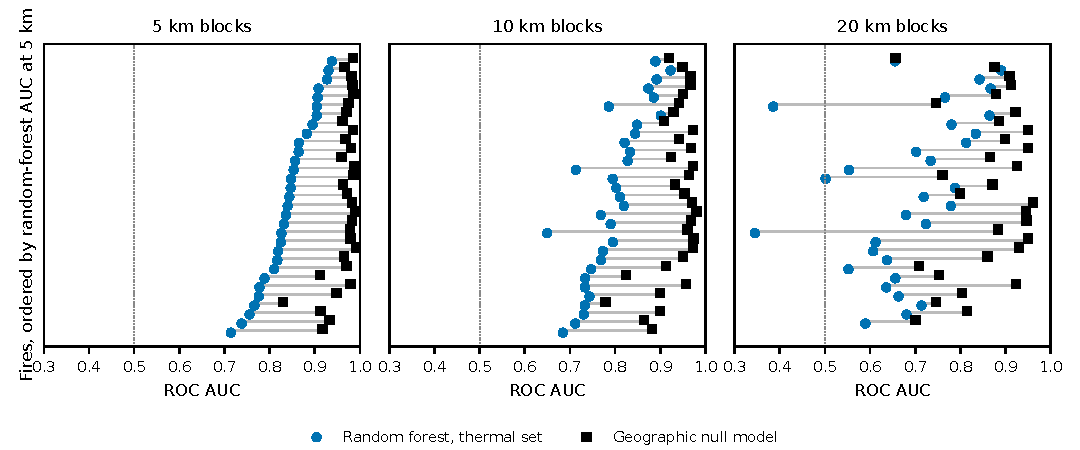
\includegraphics[width=\linewidth]{figures/Figure_1.pdf}
\caption{ROC AUC of the geographic null model (black squares) and of the thermal random forest (blue circles) in each fire, for three block sizes. Each row is one fire, ordered by the forest's AUC, and the grey line joins the two scores of that fire. The dotted line marks AUC 0.5.}
\label{fig:pairs}
\end{figure}

Distance matching took the null model to \vpwdNullFive{} on the kept pairs, close to chance as intended. On the same pairs the thermal forest reached a calibrated AUC of \vcaucFive{} [\vcaucFiveLo, \vcaucFiveHi], against \vcaucBaseFive{} for the baseline set. Buffering the training data had a similar effect. A 2~km buffer lowered the forest to \vbufRfTwo{} and the null model to \vbufNullTwo{}, and a 5~km buffer to \vbufRfFive{} and \vbufNullFive{}. At 10~km so few burned training cells remained that \vbufSkipTen{} of \vbufFolds{} folds could not be fitted.

\subsection{Distance bands}
\label{sec:res-bands}

With the predictions fixed, the forest's AUC rose from \vbandARf{} [\vbandARfLo, \vbandARfHi] when the unburned cells lay within 0.5~km of the fire to \vbandFRf{} [\vbandFRfLo, \vbandFRfHi] beyond 10~km (Fig.~\ref{fig:bands}). The rise of \vrise{} [\vriseLo, \vriseHi] was positive in \vriseFires{} fires, and in \vriseFiresHgb{} for gradient boosting. The null model followed a steeper curve. It was below the forest only in the nearest band, where the forest led in \vbandARfWins{} fires, level with it between 0.5 and 1~km and far above it from 1~km on. Environmental distance gave the same pattern, with an AUC of \venvQone{} for the unburned cells most similar to the burned ones and \venvQfive{} for the least similar.

\begin{figure}[t]
\centering
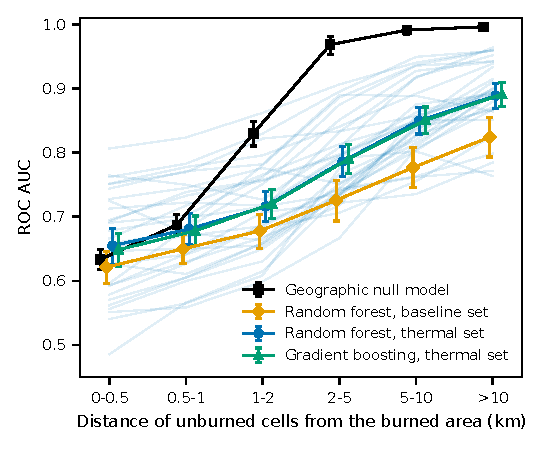
\includegraphics[width=0.6\linewidth]{figures/Figure_2.pdf}
\caption{ROC AUC by distance band of the unburned cells, with the out-of-fold predictions of the 5~km design held fixed. Markers are means over the 31 fires and bars their 95\% bootstrap intervals, offset sideways so that all four models stay visible. Thin blue lines are the thermal random forest in single fires.}
\label{fig:bands}
\end{figure}

\subsection{Edge labels}
\label{sec:res-labels}

Sentinel-2 confirmed that MCD64A1 misses some burned area at the edge. With the stricter threshold, \vlerrA\% [\vlerrALo, \vlerrAHi] of the unburned cells in the nearest band were at least half burned, against \vlerrF\% beyond 10~km (Fig.~\ref{fig:labels}). The looser threshold of 0.10 flagged \vlerrTenFarBand\% of the farthest cells as burned, which points to dry-season browning more than fire, so we read the stricter one. Removing the ambiguous cells moved the nearest band from \vnearMcd{} to \vnearDrop{} and closed \vclosedDrop\% of the gap to the farthest band. Relabelling the missed cells as burned lowered it to \vnearRelabel{}. The relabelled cells were thus as hard for the model as the rest, and the decision rule kept the band result.

\begin{figure}[t]
\centering
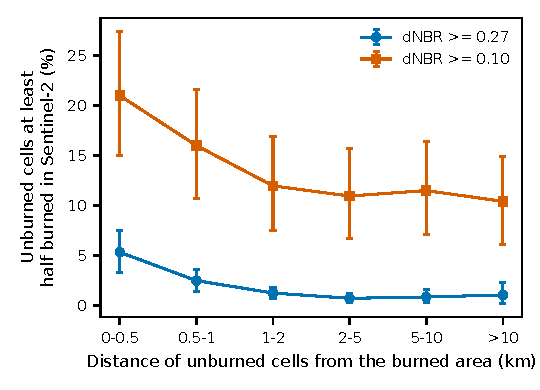
\includegraphics[width=0.6\linewidth]{figures/Figure_3.pdf}
\caption{Share of the cells that MCD64A1 labels unburned but Sentinel-2 maps as at least half burned, by distance band, for two differenced Normalised Burn Ratio thresholds. Markers are means over fires and bars their 95\% bootstrap intervals.}
\label{fig:labels}
\end{figure}

\subsection{Multi-year label}
\label{sec:res-multiyear}

With all burns from 2001 to 2023 as the label (\vmyBurned\% of cells burned on average), the null model scored \vmyNull{} against \vmyRf{} for the forest and led in \vmyWins{} fires at 5~km and \vmyWinsTen{} at 10~km. This is below the 28 fires the plan set for the first claim, so that claim holds in full for single-event labels and in most fires for multi-year ones. The calibrated AUC was \vmyCauc{} and the distance rise \vmyRise{}, positive in \vmyRiseFires{} fires. A label built only from burns before the fire gave a similar picture (\vhistWins{} fires).

\subsection{Published datasets}
\label{sec:res-open}

Table~\ref{tab:open} and Fig.~\ref{fig:open} compare the null model with the AUC reported for each dataset. Under the Alberta temporal test, with training up to 2014 and testing on 2018 to 2021, the null model reached \valTempNull{}, above the best of the four published models (\valTempRep). In British Columbia it reached \vbcNull{} against 0.92 reported and \vbcRf{} for our forest on the same folds. On the Mesogeos test years it reached an AUC of \vmeNull{} and a PR-AUC of \vmeNullPr{} at a prevalence of \vmePrev{}. The null model fell behind with the Korean ignition points under a random split (\vkoNull{} against \vkoRep{}), with 100~km blocks in Alberta (\valBlockNull{} against \valBlockRep{}) and most of all in Italy, where \vitFolds{} regional blocks left it at \vitNull{} while our forest reproduced \vitRf{} against \vitRep{} reported.

\begin{table}[t]
\centering
\caption{The geographic null model on five published datasets, scored on the authors' test data under their own validation design. Our random forest on the same split is given where the package contains the predictors.}
\label{tab:open}
\small
\begin{tabular}{llccc}
\toprule
Dataset & Validation & Reported AUC & Our forest & Null model \\
\midrule
Alberta & Temporal, test 2018--2021 & \valTempRep & -- & \valTempNull \\
British Columbia & 50 km blocks, 10 folds & 0.92 & \vbcRf & \vbcNull \\
Mesogeos & Temporal, test 2021--2022 & PR-AUC 0.85 & -- & \vmeNull \\
South Korea & Random 70/30 & \vkoRep & \vkoRf & \vkoNull \\
Alberta & 100 km blocks, 5 folds & \valBlockRep & -- & \valBlockNull \\
Italy & Regional blocks, \vitFolds{} folds & \vitRep & \vitRf & \vitNull \\
\bottomrule
\end{tabular}
\end{table}

\begin{figure}[t]
\centering
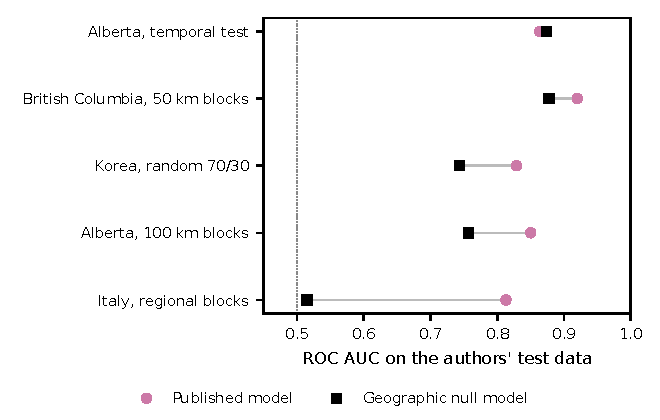
\includegraphics[width=0.7\linewidth]{figures/Figure_4.pdf}
\caption{Reported ROC AUC of the published model (pink circles) and AUC of the geographic null model (black squares) on the same test data, for the datasets that report ROC AUC. The dotted line marks AUC 0.5.}
\label{fig:open}
\end{figure}

\subsection{Transfer and pre-fire temperature}
\label{sec:res-secondary}

A forest trained on one fire scored \vtrRaw{} [\vtrRawLo, \vtrRawHi] on average over the \vtrDirections{} ordered pairs of fires, \vtrZ{} with standardised predictors and \vtrMinmax{} with min-max scaling. Single-fire transfer scored about the same in the nearest band of the target (\vtrNear) as in its farthest band (\vtrFar). Four label-free similarity measures (distance between fires, same year, domain-classifier AUC and mean shift of the predictors) did not predict the transfer score, with Spearman's $\rho$ between \vrhoShift{} and \vrhoYear{} and every interval including zero. A model pooled from the other 30 fires with standardised predictors reached \vtrPoolZ{} [\vtrPoolZLo, \vtrPoolZHi], \vtrPoolZNear{} in the nearest band and \vtrPoolZFar{} in the farthest. The learning curve rose from \vcurveFirst{} with two source fires to \vcurveTen{} with ten and \vcurveLast{} with \vcurveLastK{} (Fig.~\ref{fig:curve}).

\begin{figure}[t]
\centering
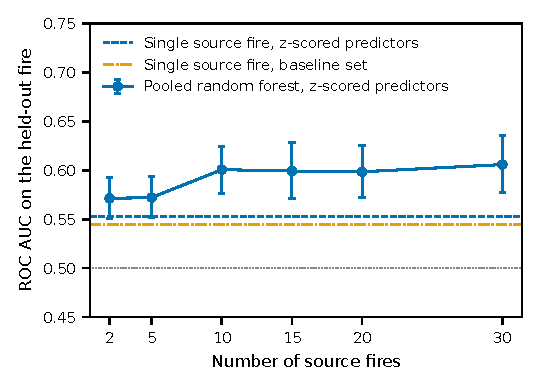
\includegraphics[width=0.6\linewidth]{figures/Figure_5.pdf}
\caption{ROC AUC on a held-out fire of a random forest pooled from a growing number of source fires, with predictors standardised within each fire. Markers are means over target fires and bars their 95\% bootstrap intervals. The dashed line is the mean of single-fire transfer with raw predictors and the dotted line marks AUC 0.5.}
\label{fig:curve}
\end{figure}

Burned cells were cooler before the fire than unburned ones in \vlstCool{} fires for the morning Landsat LST (AUC \vlstAuc{} [\vlstAucLo, \vlstAucHi]), with intervals entirely below 0.5 in \vlstCoolCi{} fires and above it in \vlstHotCi{}. The afternoon Aqua LST, which correlated with the morning LST at \vlstCorr{}, gave \vaquaCool{} fires and an AUC of \vaquaAuc{}. After removing elevation, NDVI, tree cover and aspect, the direction held in \vlstCoolCtl{} fires for the morning LST and \vaquaCoolCtl{} for the afternoon LST.

\section{Discussion}
\label{sec:discussion}

The geographic null model scored higher than the predictor-based models in every fire, and their AUC depended on how far the test negatives lay from the fire. Section~\ref{sec:disc-meaning} discusses what the null model measures, Section~\ref{sec:disc-lit} relates the results to earlier work, Section~\ref{sec:disc-protocol} turns them into recommendations and Section~\ref{sec:disc-limits} gives the limits of the study.

\subsection{What the null model measures}
\label{sec:disc-meaning}

The null model is not a forecasting tool, since it needs the labels of neighbouring blocks. It measures how much of a score the validation design hands to any model that knows where the training fires are. With 5~km blocks inside one fire, a test cell almost always has burned training cells within a few kilometres, and closeness alone separates the classes. The forest learns the same thing through predictors that vary smoothly in space, which is why its AUC falls to \vcaucFive{} once distance is matched and why it rises with the distance of the negatives. The bands show where the predictors add something. Within 0.5~km of the fire the forest beat the null model in \vbandARfWins{} fires, and beyond 1~km it never did. The thermal predictors raised the calibrated AUC by \vcaucGain{} over the baseline set, a real but small gain next to the gap of \vcaucGap{} between the usual AUC and the calibrated one.

The open datasets show that this is a property of the design. Under the Alberta temporal test, closeness to the fires of earlier years was as good as four published models trained on 16 predictors sampled in patches of 5 by 5 cells, while under the Italian regional blocks it was close to chance. The same predictor-free score thus reads as a diagnosis of the split. Where it is high, a reported AUC says more about the spatial clustering of fires than about the predictors.

\subsection{Comparison with earlier work}
\label{sec:disc-lit}

The mechanism is the spatial sorting bias of \citet{Hijmans2012} and the spatial dependence discussed by \citet{Roberts2017}, \citet{Meyer2018} and \citet{Ploton2020}. In those studies the null model or the coordinate-only model matched or beat environmental models in part of the cases. Our fires are a more extreme case, with the null model ahead in all 31, which fits the fact that one fire scar is a single contiguous patch. The distance profile is close to the prediction-distance profiles of \citet{Brenning2023} and \citet{Frank2025}, who plotted regression error against the distance to the nearest training point. The bands here differ in that the model and the training data stay fixed and only the negatives change, so the profile isolates the evaluation from the fit. The rise from 0.66 to 0.89 matches the direction of \citet{Zerouali2026} at a larger scale. A landslide study found almost flat AUC across buffers of 0.1 to 5~km \citep{Xiao2026}, so the size of the effect depends on how quickly the landscape changes away from the event.

For transfer, raw scores near 0.5 agree with the four-fire results of \citet{Stark2026} and \citet{Bekar2020} more than with the mean of about 0.84 in the pairwise table of \citet{Dimarco2026}, who used the same burned-area product and similar scaling. Their targets were whole regions with many distant negatives, which favours the farthest-band case. In our fires only the pooled model scored higher in the farthest band (\vtrPoolZFar) than in the nearest one (\vtrPoolZNear), and single-fire transfer stayed near chance in both, so the distance of the negatives explains part of the gap at most. The cooler pre-fire surfaces of burned cells run against most published results \citep{Maffei2018,ParkSim2023} and agree with an isolated negative coefficient in \citet{Das2023}. A likely reading is that forests are cooler and carry more fuel, although the direction held after controlling for tree cover and aspect in most fires.

\subsection{Recommendations}
\label{sec:disc-protocol}

Three additions to a susceptibility study would make its AUC readable. The first is to report the geographic null model under the same split, which costs one nearest-neighbour query per fold. The second is to report the calibrated AUC next to the usual one. The third is to report the AUC of the fixed predictions by distance band, or at least within 1~km of the fire, which is where a susceptibility map is used to choose between neighbouring stands. A score that does not beat the null model, or beats it only far from the fire, should not be read as evidence that the predictors capture fire risk. The analysis code is released so that the three numbers can be added to an existing study with its own data and folds.

\subsection{Limitations}
\label{sec:disc-limits}

The 26 added fires were selected and windowed by rule, without the manual checks given to the five earlier regions. In \vexclCount{} of them more than 20\% of cells missed a thermal predictor, and excluding these left \vexclNullWins{} fires won by the null model. The study uses one burned-area product at 500~m and two tree ensembles. The Sentinel-2 check found that the looser threshold confuses browning with burning, so the label check rests on the stricter threshold. The multi-year result fell short of the pre-registered count, and the claim for inventories rests on a majority of fires. The open datasets are five, chosen because they could be rebuilt, and two of them lack predictors, so our forest could not be checked there. The pre-fire temperature result is an association, and the overpass time, fuel moisture and canopy structure that could explain it were not measured.

\section{Conclusions}
\label{sec:conclusions}

A wildfire susceptibility model can reach a high AUC without learning much about fire, because burned cells cluster and test negatives lie far from them. On 31 Mediterranean fires a model with no predictors beat a random forest in every fire, and the forest's AUC fell from \vaucRfFive{} to \vcaucFive{} once distance was matched. The checks with Sentinel-2 labels, a multi-year label and five published datasets limit the claim but do not remove it. We recommend that susceptibility studies report the geographic null model, the calibrated AUC and the distance-banded AUC with their results. Future work should test the protocol on other fire regimes and on ignition data, and use the near-fire bands to compare predictors that may help where the null model cannot.

\section*{Software and data availability}

Software name: thermal-twin analysis code (scale-up branch). Developers: Y.E. Cogurcu and E. Metin, ycogurcu@cu.edu.tr. First available: 2026. Hardware: a desktop computer with 32 threads. Software required: Python 3.12 with NumPy, pandas, SciPy, scikit-learn, rasterio and the Earth Engine Python API. Programming language: Python. Availability and cost: free, MIT licence, at https://github.com/dryuemco/thermal-twin, archived at Zenodo \citep{ThermalTwinRepo}. The upstream processing pipeline is at https://github.com/emrehann17/satellite-thermal-digital-twin. All satellite inputs are public and were accessed through Google Earth Engine. The modelling tables of the 31 fires, the Sentinel-2 and multi-year label rasters and every number in this paper are released with the code. The five published datasets are available from their own repositories \citep{Heo2026data,Alberta2026data,Khan2026data,Cilli2023data,Mesogeos2025data}.

\section*{CRediT authorship contribution statement}

Emrehan Metin: Software, Data curation, Investigation, Validation, Writing -- review and editing. Yunus Emre Cogurcu: Conceptualization, Methodology, Formal analysis, Investigation, Visualization, Writing -- original draft, Writing -- review and editing, Supervision, Project administration, Funding acquisition.

\section*{Declaration of competing interest}

The authors declare that they have no known competing financial interests or personal relationships that could have appeared to influence the work reported in this paper.

\section*{Funding}

This work was supported by the \c{C}ukurova University Scientific Research Projects Coordination Unit under project FKB-2025-17608. The funder had no role in the study design, the analysis, the writing or the decision to submit.

\section*{Declaration of generative AI and AI-assisted technologies in the manuscript preparation process}

During the preparation of this work the authors used Claude (Anthropic) to write analysis and figure code, to check reported numbers and to edit the language. After using this tool, the authors reviewed and edited the content as needed and take full responsibility for the content of the published article.

\section*{Acknowledgements}

The authors thank the Department of Computer Engineering at \c{C}ukurova University for the laboratory environment in which this work was carried out.

\bibliographystyle{elsarticle-harv}
\bibliography{references}

\end{document}
